\chapter{Prezentacja warstwy użytkowej projektu}
\label{ch:widoki}

W tym rozdziale prezentowana jest wizualna część aplikacja Rock Gym. Opisane są kluczowe widoki i scenariusze korzystania z nich przez personel.

\section{Logowanie i Panel Główny}

\subsection{Logowanie do systemu}
Prezentacja ekranu logowania obejmuje podstawowy wygląd formularza, wymagającego podania nazwy użytkownika oraz hasła, wraz z bezpieczną obsługą błędów w przypadku wpisania nieprawidłowych danych.

\begin{figure}[H]
    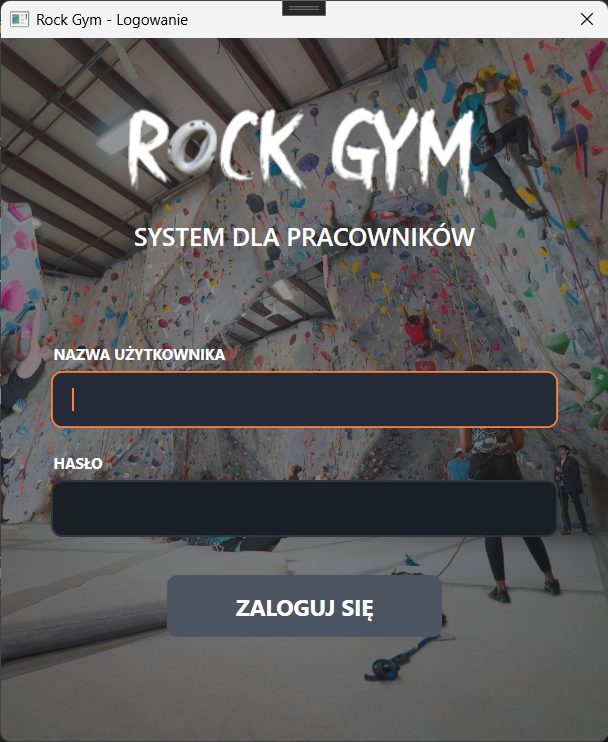
\includegraphics[width=0.45\textwidth]{figures/widoki/LoginView.png}
    \hfill
    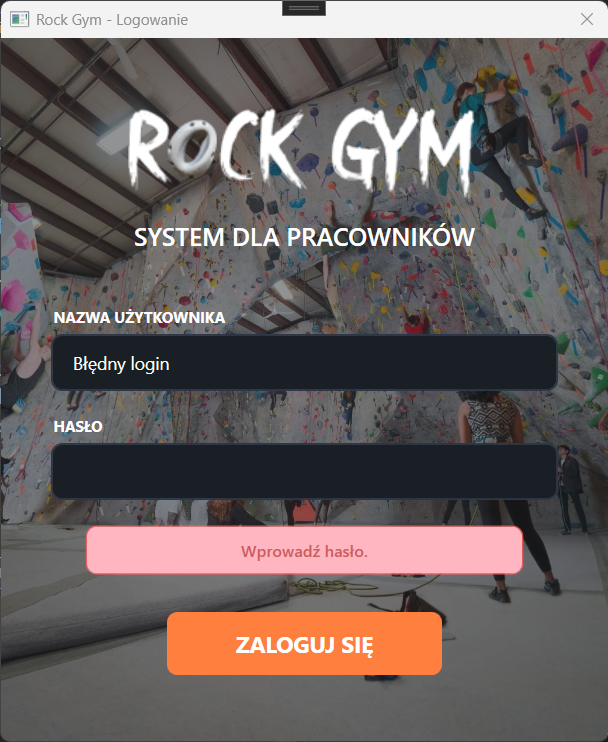
\includegraphics[width=0.45\textwidth]{figures/widoki/LoginView_error.png}
    \caption{Ekran logowania do systemu i ekran logowania z błędnymi danymi}
    \label{fig:login_view}
\end{figure}


\subsection{Panel główny i różnice w uprawnieniach}
Struktura okna głównego zmienia się w zależności od posiadanych uprawnień. Po pomyślnym zalogowaniu na konto menedżera (administratora) użytkownik posiada dostęp do pełnej nawigacji. Z kolei na koncie pracowniczym część elementów, takich jak menu podsumowania, zostaje ukryte.

\begin{figure}[H]
    \centering
    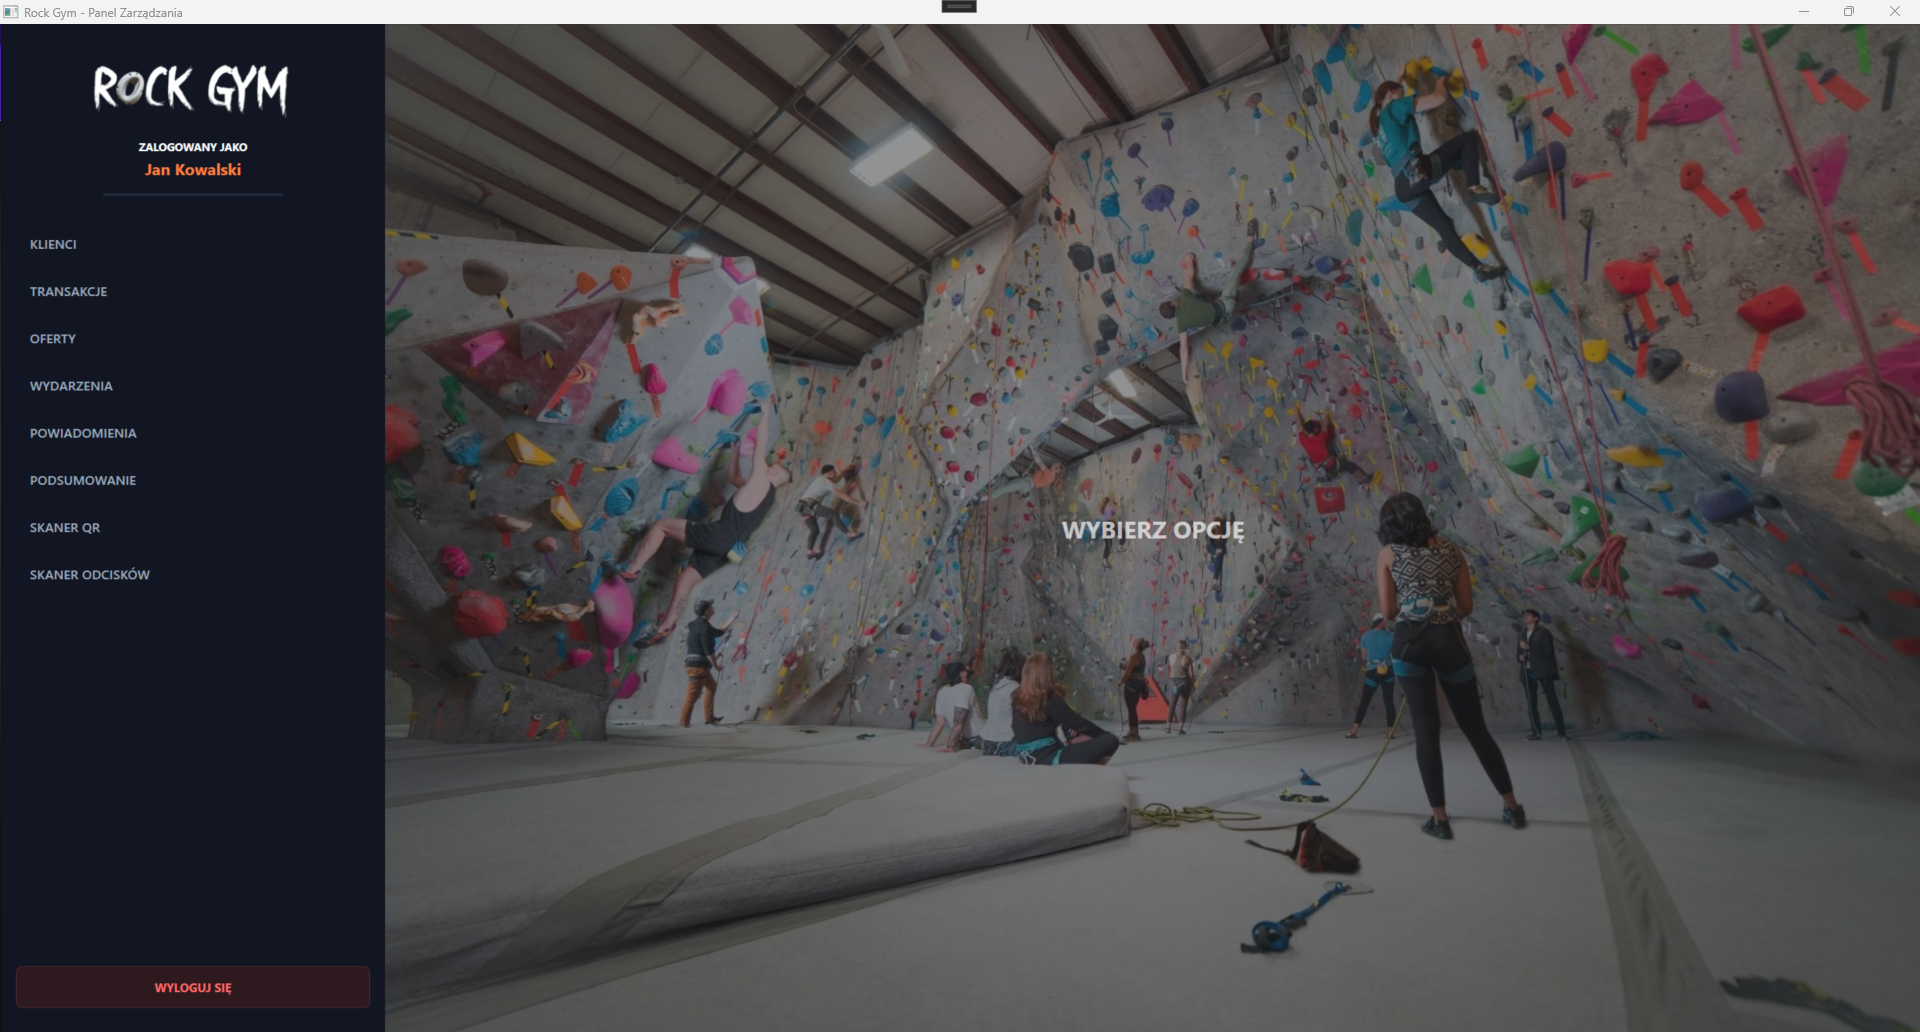
\includegraphics[width=0.9\textwidth]{figures/widoki/MainWindow_admin.png}
    \caption{Widok główny dla konta administratora (pełen dostęp)}
    \label{fig:main_admin}
\end{figure}

\begin{figure}[H]
    \centering
    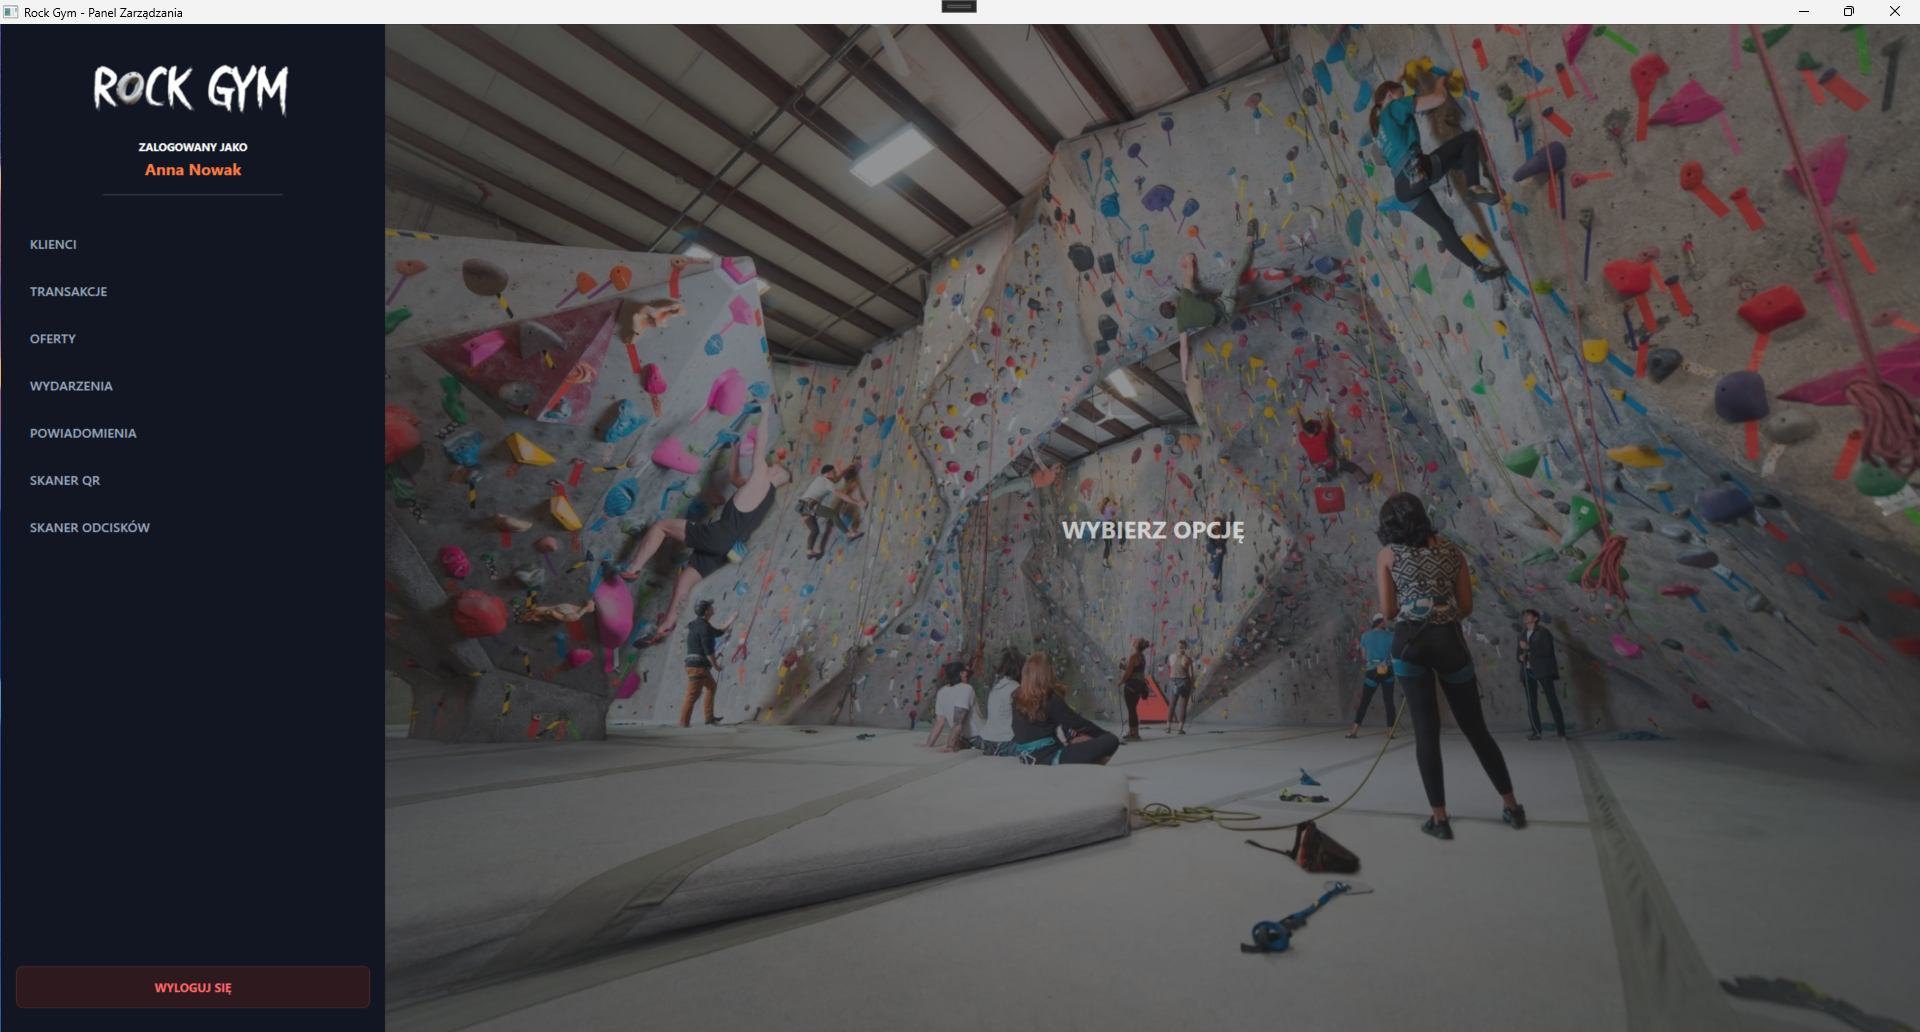
\includegraphics[width=0.9\textwidth]{figures/widoki/MainWindow_pracownik.png}
    \caption{Widok główny dla konta pracowniczego (ograniczony dostęp)}
    \label{fig:main_pracownik}
\end{figure}

\subsection{Pulpit podsumowujący}
Opis widoku zbiorczego prezentującego statystyki i najważniejsze aktualne informacje z obiektu. Moduł ten jest dedykowany i dostępny wyłącznie dla menadżerów. Menadżer może tu sprawdzić miesięczny utarg, liczbę transakcji z dzisiaj lub miesiąca i wiele innych. Można też zmieniać datę, dla której wyświetlane są statystyki. Menadżer ma też możliwość pobrania wszystkich wyciągów ze wszystkich transakcji jako plik \texttt{.xlsx}.

\begin{figure}[H]
    \centering
    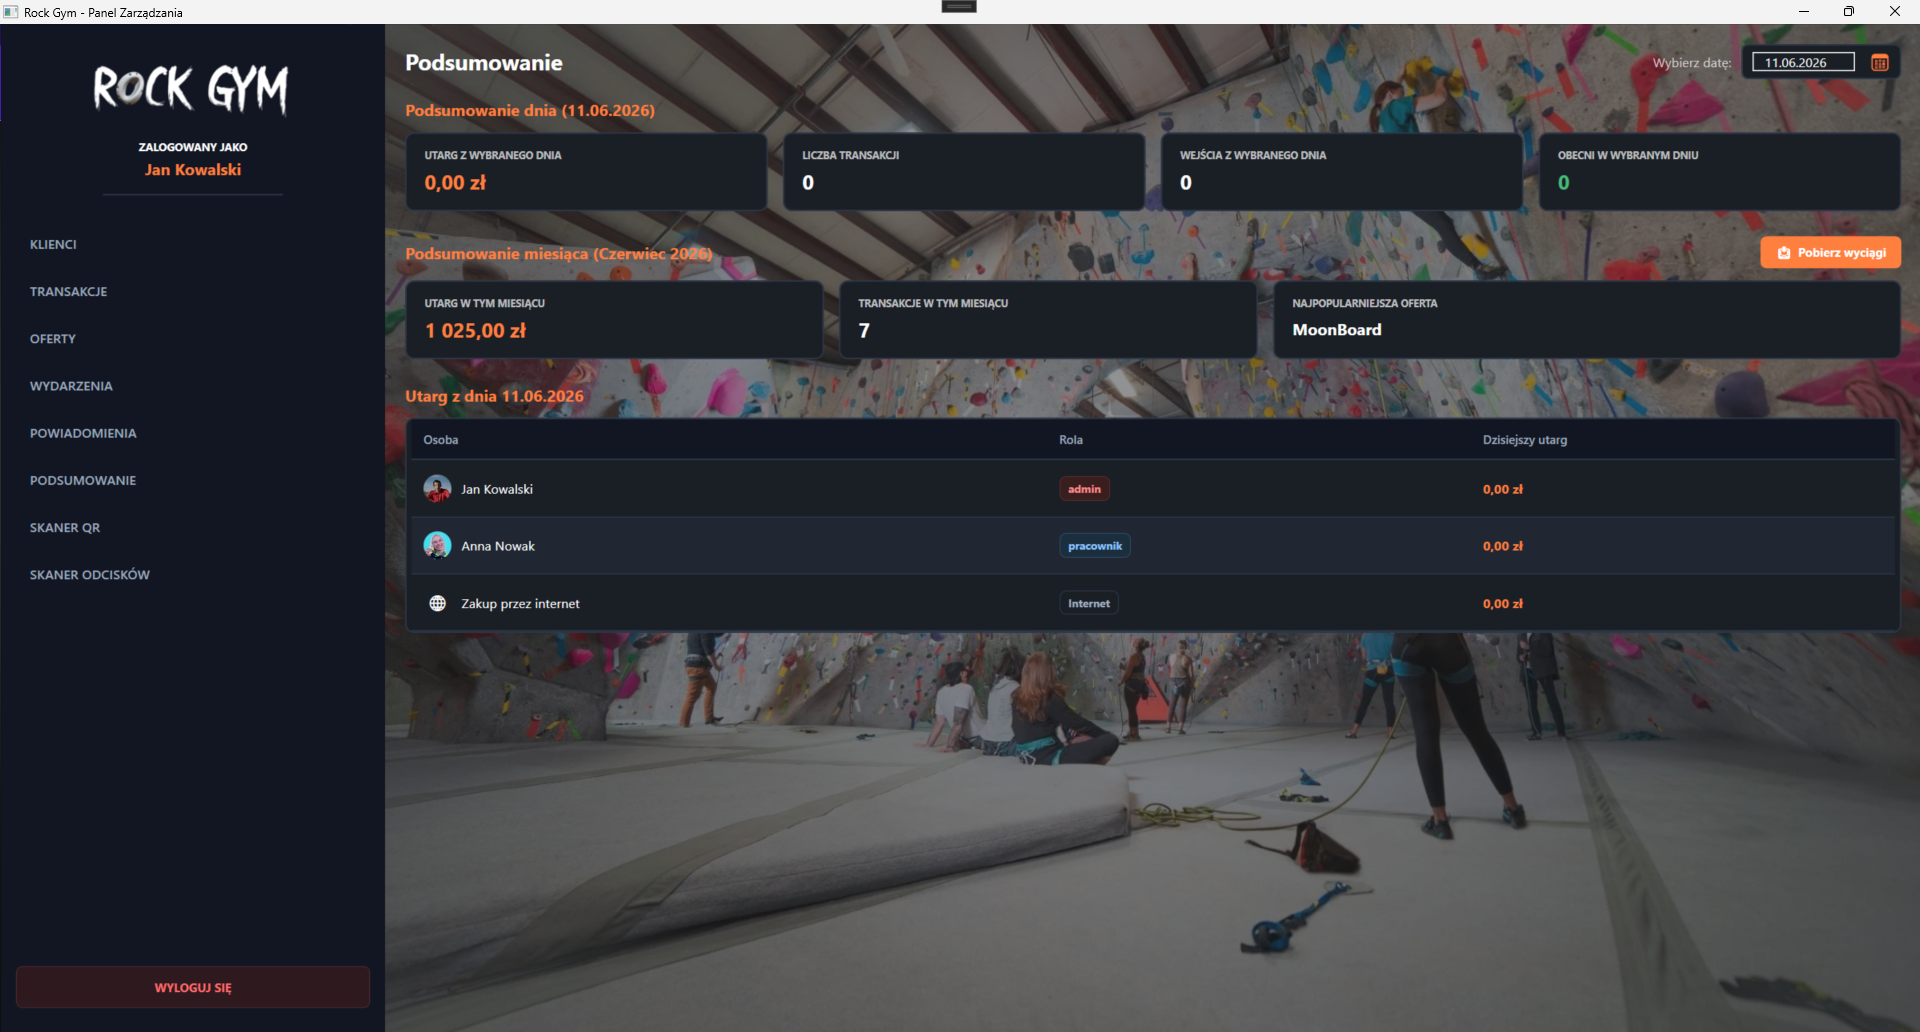
\includegraphics[width=0.9\textwidth]{figures/widoki/SummaryView.png}
    \caption{Pulpit podsumowujący najważniejsze informacje}
    \label{fig:summary_view}
\end{figure}

\section{Zarządzanie danymi i funkcje modułów}
Aplikacja podzielona została na odrębne zakładki pozwalające realizować operacje CRUD. Nowe rekordy dodawane i edytowane są za pomocą wyskakujących okien modalnych.

\subsection{Zarządzanie klientami i personelem}
Z poziomu głównej tabeli użytkowników możliwy jest wgląd we wszystkie zarejestrowane osoby. Aplikacja ułatwia pracę poprzez wbudowaną wyszukiwarkę filtrującą bazę po imieniu i nazwisku. W tym module występują wyraźne różnice w uprawnieniach -- pracownik z podstawowymi uprawnieniami, nie może usuwać innych użytkowników oraz ma zablokowaną możliwość edycji kont o statusie menadżera.
Z poziomu edycji użytkownika, oprócz zmiany danych tekstowych, pracownik może również wejść w dedykowane panele, by wygenerować nowy kod QR klienta (do autoryzacji wejść na obiekt) lub dodać nowy wzorzec odcisku palca.

\begin{figure}[H]
    \centering
    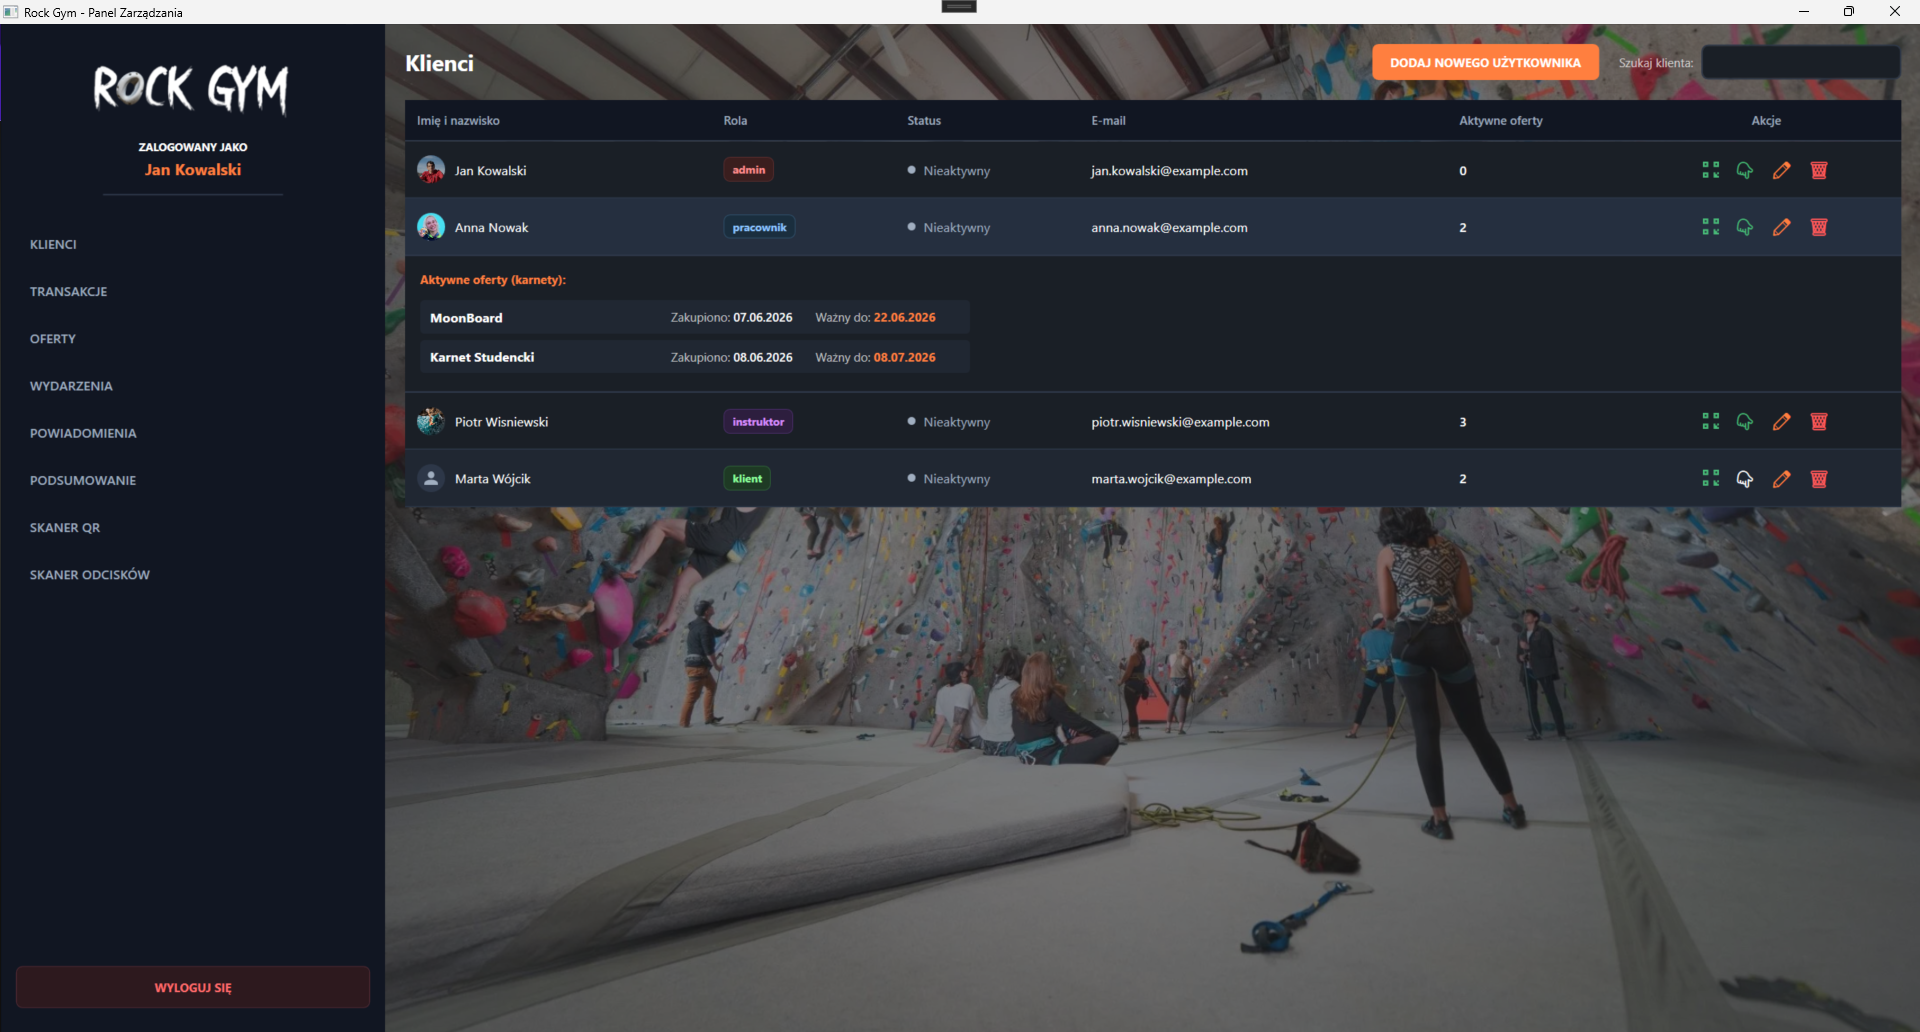
\includegraphics[width=0.9\textwidth]{figures/widoki/CustomerView_admin.png}
    \caption{Zarządzanie bazą klientów i personelu}
    \label{fig:customer_view}
\end{figure}

\begin{figure}[H]
    \centering
    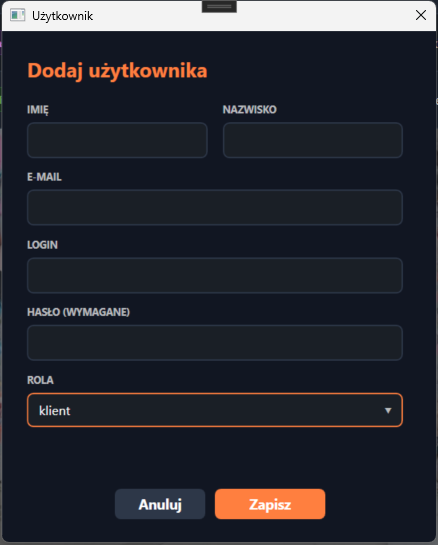
\includegraphics[width=0.6\textwidth]{figures/widoki/UserEditWindow_add.png}
    \caption{Formularz dodawania nowego użytkownika}
    \label{fig:user_add}
\end{figure}

\subsection{Wydarzenia}
Panel obsługujący listę nadchodzących zajęć i wydarzeń na obiekcie. Menadżer ma pełny dostęp do podglądu wszystkich wydarzeń, a także możliwość ich tworzenia. Zwykły pracownik ma uprawnienia wyłącznie do przeglądania zajęć, które jeszcze się nie odbyły (brak możliwości dodawania lub widoku dawnych zdarzeń).

\begin{figure}[H]
    \centering
    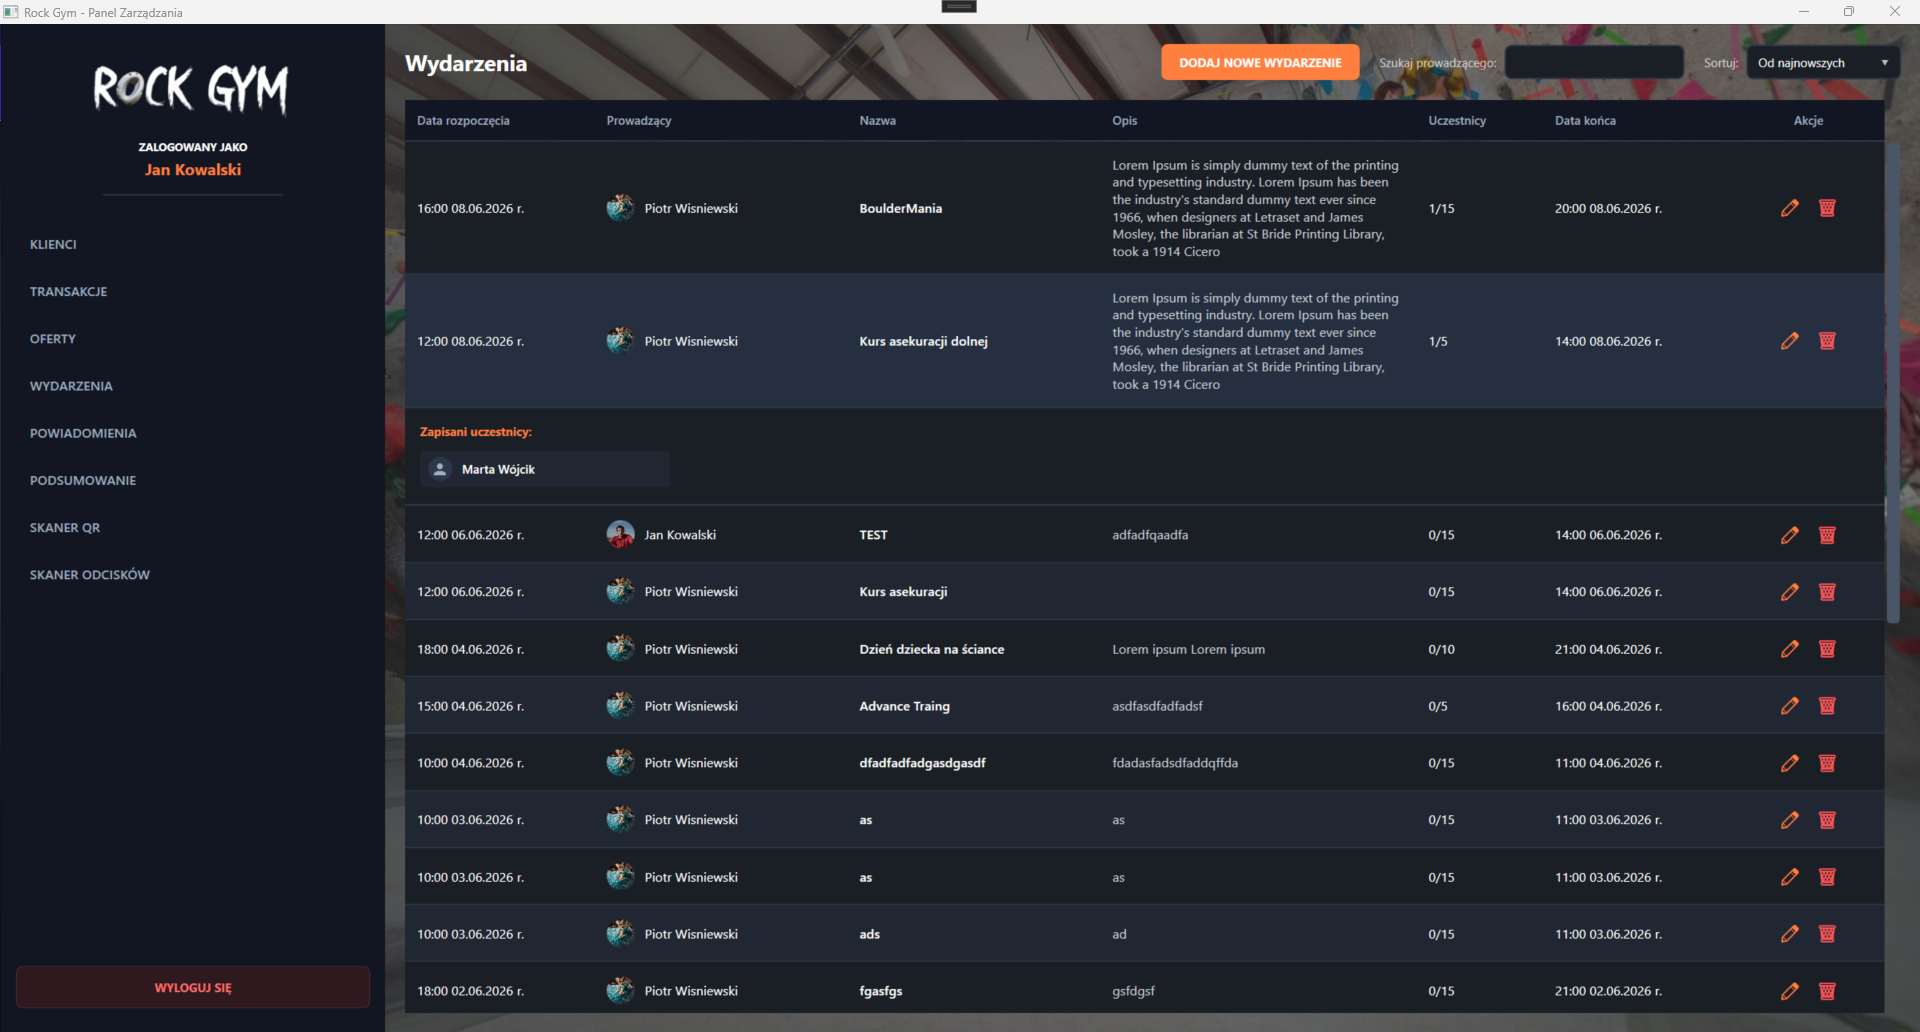
\includegraphics[width=0.9\textwidth]{figures/widoki/EventView.png}
    \caption{Widok kalendarza/tabeli zaplanowanych zajęć}
    \label{fig:event_view}
\end{figure}

\subsection{Oferta i cennik}
Zestawienie aktualnych usług oraz karnetów na ściance. Analogicznie do innych modułów, tylko profil menadżerski może modyfikować wpisy w cenniku lub dodawać nową ofertę, natomiast rola pracownicza posiada tu jedynie uprawnienie podglądu.

\begin{figure}[H]
    \centering
    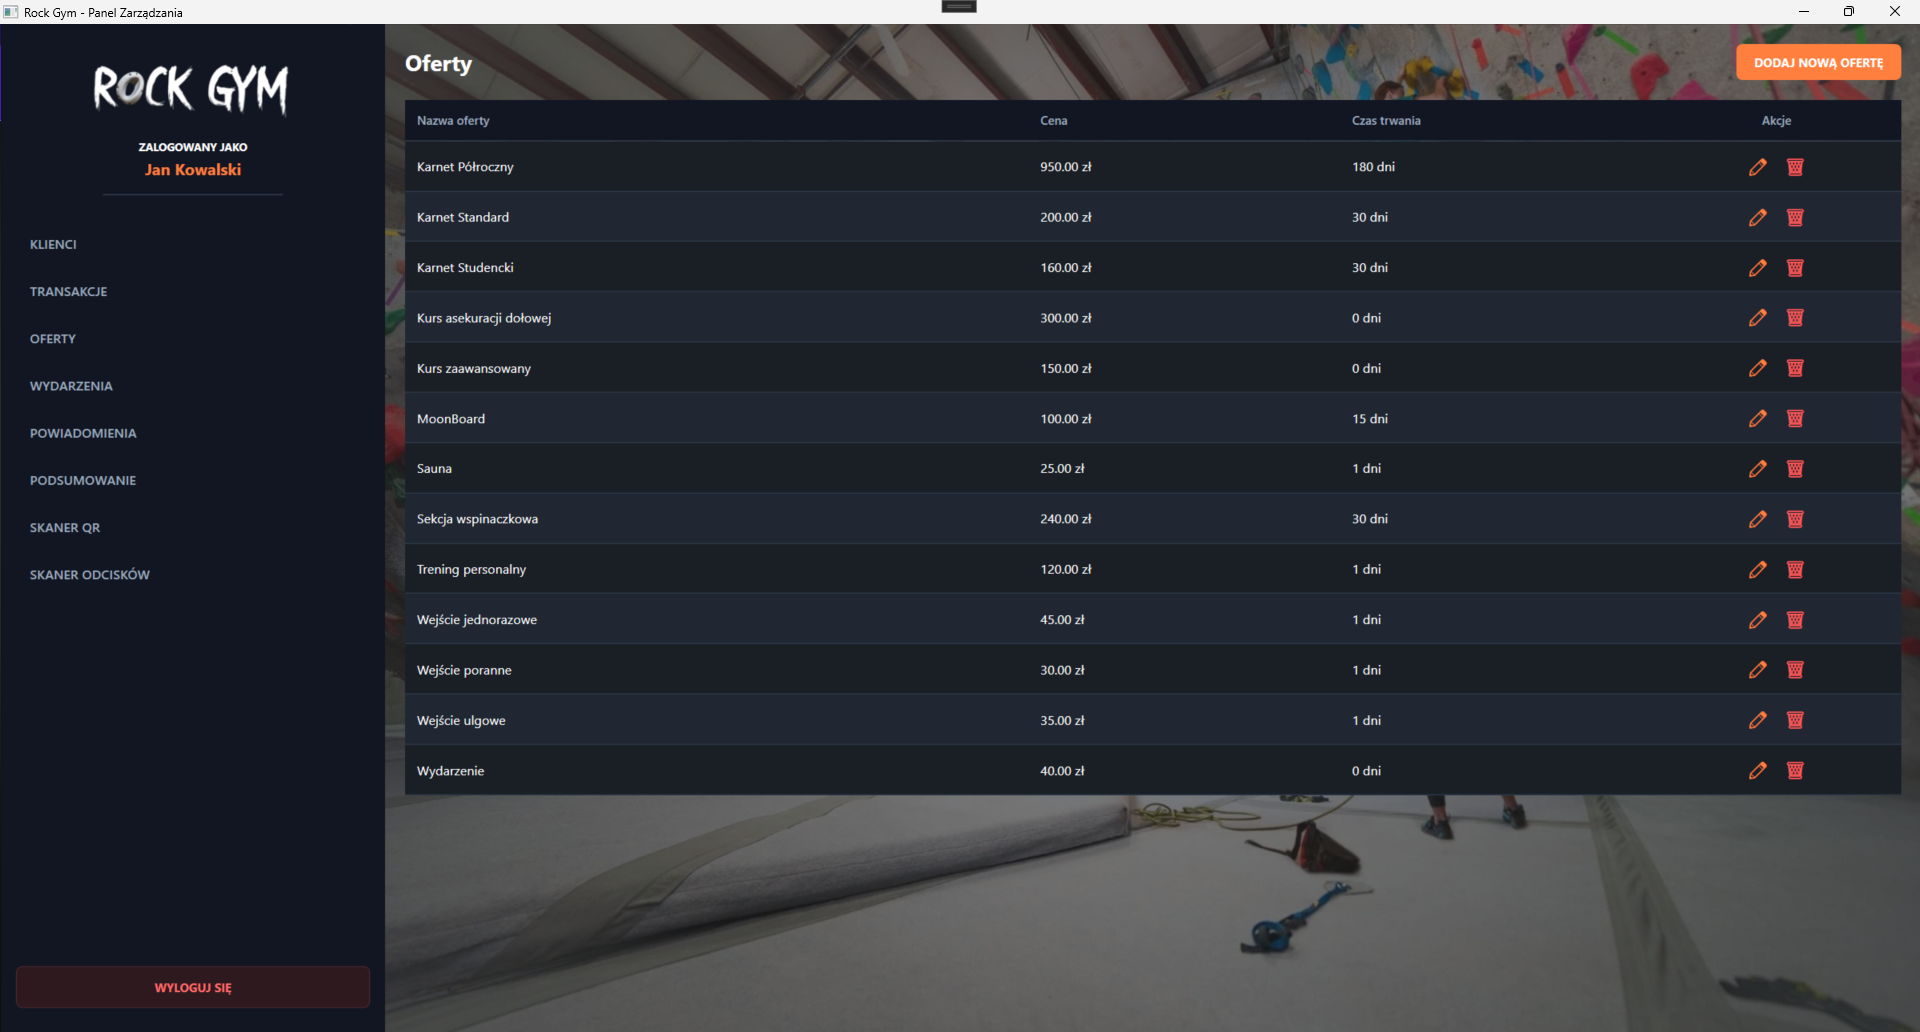
\includegraphics[width=0.9\textwidth]{figures/widoki/OfferView.png}
    \caption{Zarządzanie ofertą i typami karnetów}
    \label{fig:offer_view}
\end{figure}

\subsection{Transakcje}
Panel rozliczeń z klientami służący do tworzenia dowodów sprzedaży (np. przypisywanie zakupionych karnetów). Tabela jest domyślnie posortowana od najnowszych transakcji i umożliwia filtrowanie po imieniu oraz nazwisku kupującego. Pracownik nie ma tu praw do usuwania zaksięgowanych transakcji, ale posiada uprawnienia do ich dodawania i edycji (np. korygowania).

\begin{figure}[H]
    \centering
    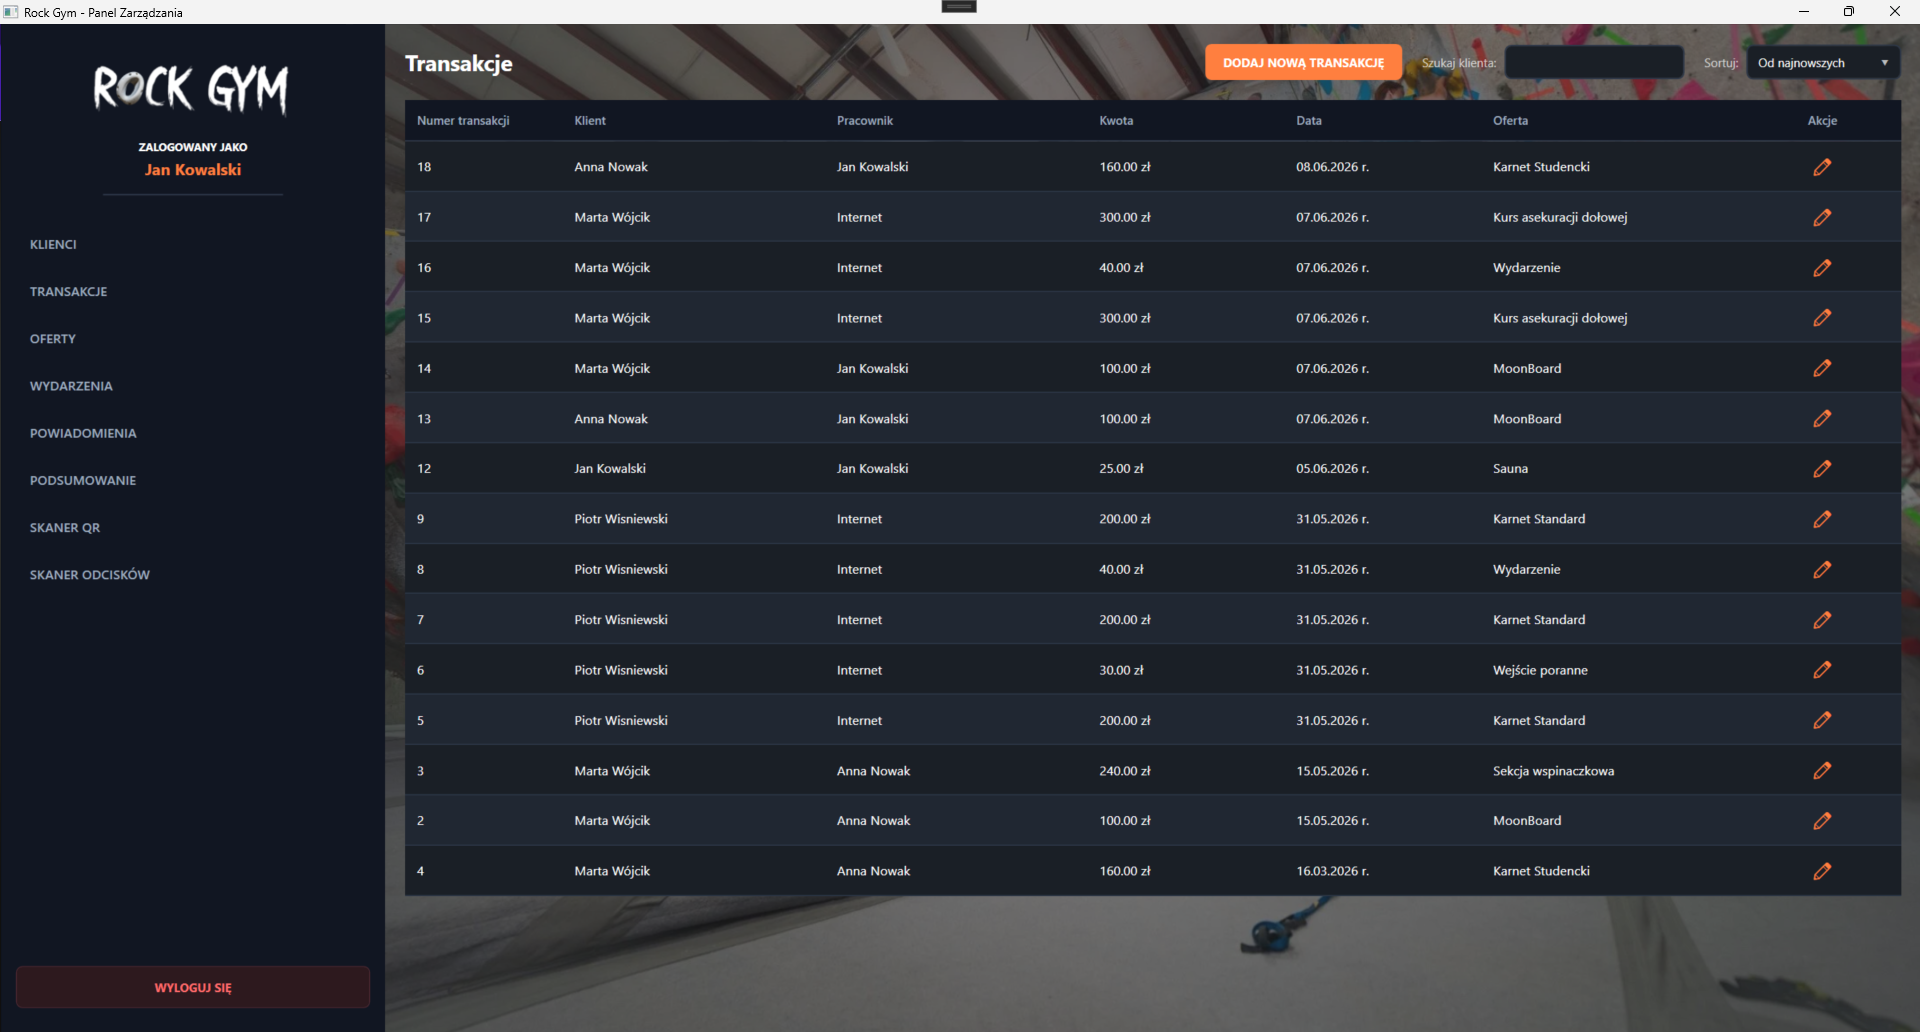
\includegraphics[width=0.9\textwidth]{figures/widoki/TransactionView.png}
    \caption{Historia transakcji na obiekcie}
    \label{fig:transaction_view}
\end{figure}

\subsection{Powiadomienia}
Wewnętrzny system usprawniający przepływ informacji. Z poziomu tej zakładki każdy pracownik widzi tablicę komunikatów i ma opcję tworzenia nowych powiadomień. Powiadomienia te wyświetlać się będą zwykłym klientom w ich aplikacji mobilnej.

\begin{figure}[H]
    \centering
    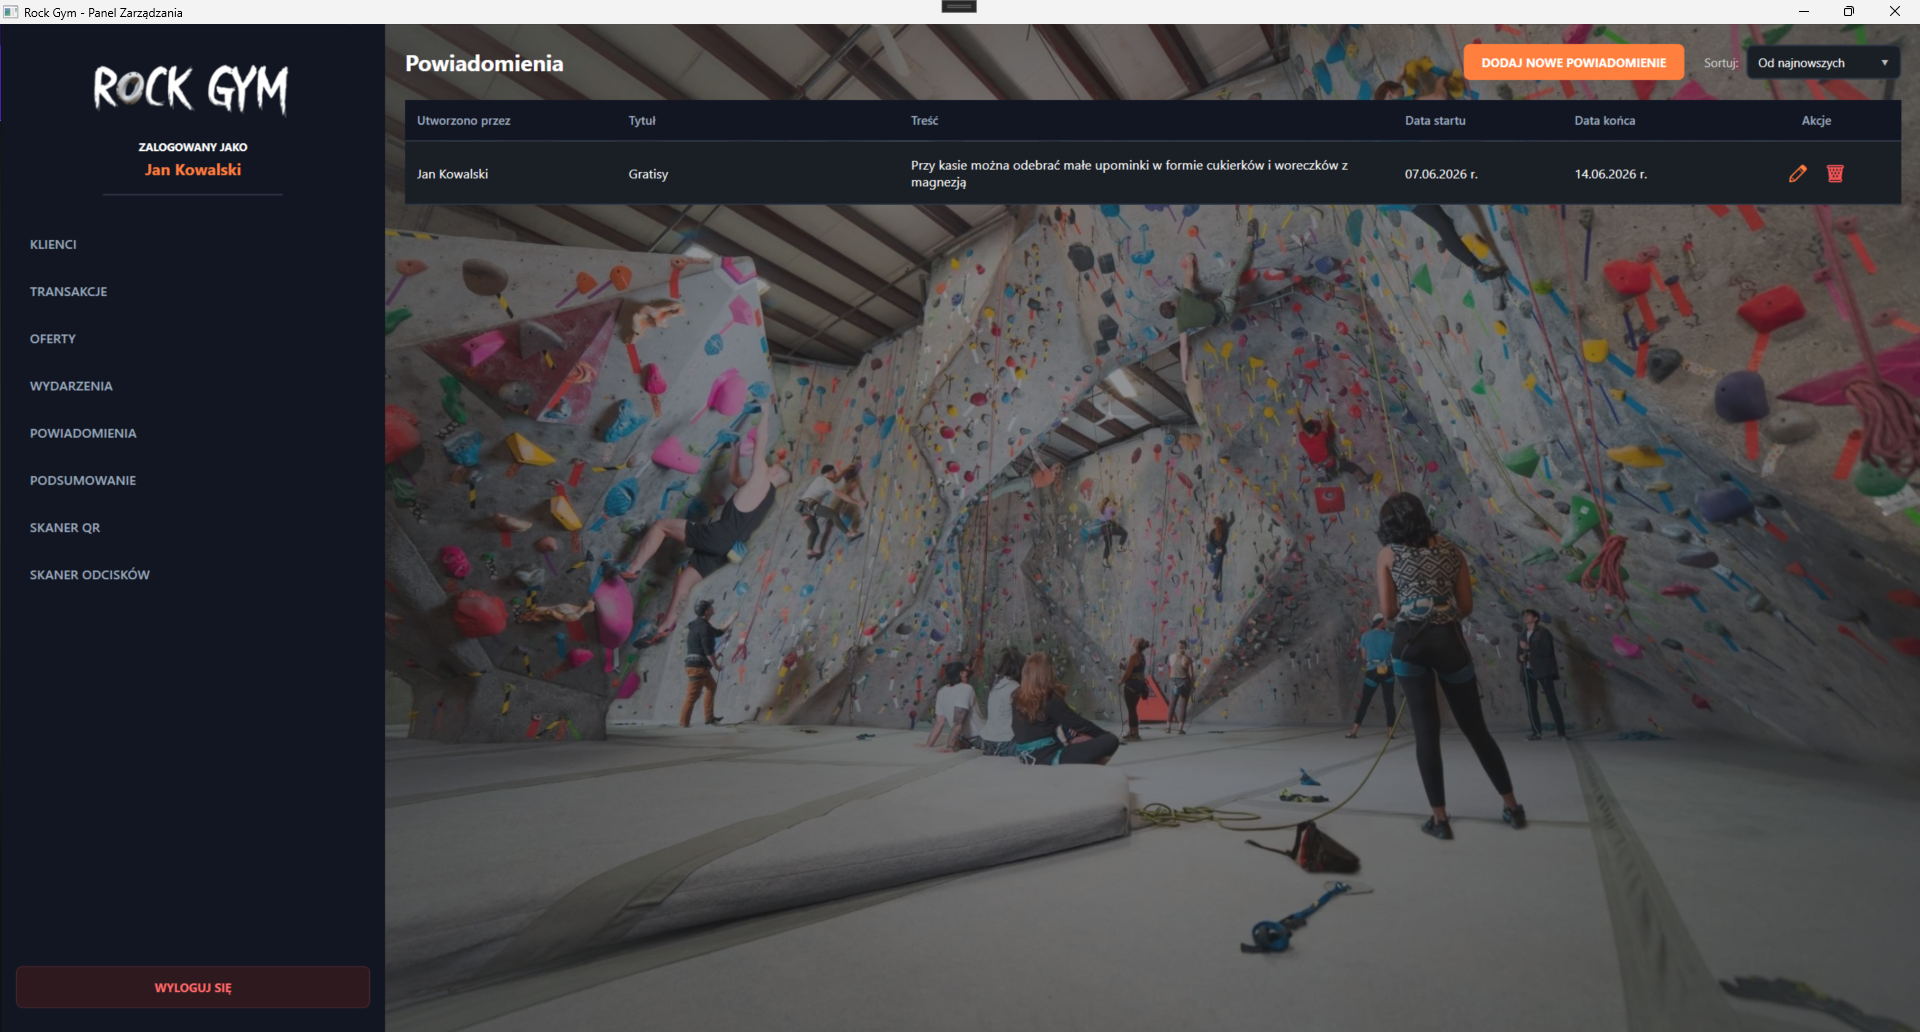
\includegraphics[width=0.9\textwidth]{figures/widoki/NotificationView.png}
    \caption{Widok panelu powiadomień}
    \label{fig:notification_view}
\end{figure}

\section{Przykładowe scenariusze działania (biometria i autoryzacja wejść)}
\subsection{Zarządzanie wzorcami biometrycznymi}
Zgodnie z koncepcją symulacji urządzenia biometrycznego, zaimplementowany proces rejestracji opiera się na wgrywaniu obrazów. Okno rejestracji odcisków pozwala pracownikowi na wskazanie pliku z odciskiem palca klienta, na podstawie którego wygenerowany zostanie hash i zapisany do bazy danych w powiązaniu z danym profilem.

\begin{figure}[H]
    \centering
    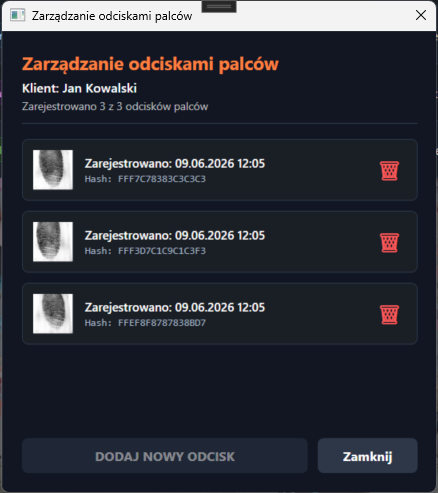
\includegraphics[width=0.3\textwidth]{figures/widoki/FingerprintManagerWindow.png}
    \caption{Menedżer dodawania odcisku palca dla klienta}
    \label{fig:fingerprint_manager}
\end{figure}

\subsection{Scenariusz 1: Wejście weryfikowane czytnikiem linii papilarnych}
Ekran startowy modułu uruchamia się w trybie oczekiwania, symulując nasłuchiwanie sprzętowego czytnika. Następnie (w ramach symulacji przyłożenia palca przez klienta) przekazywany jest plik ze zdjęciem odcisku do weryfikacji.
\begin{figure}[H]
    \centering
    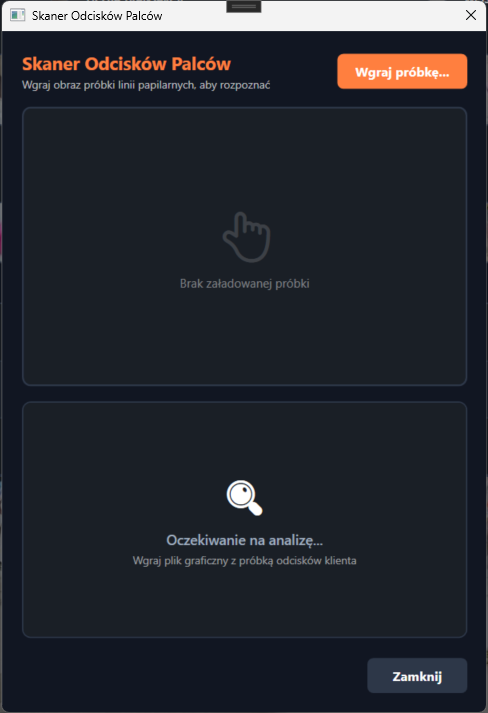
\includegraphics[width=0.40\textwidth]{figures/widoki/FingerprintScannerWindow.png}
    \caption{Czytnik linii papilarnych -- tryb oczekiwania}
    \label{fig:finger_scan_wait}
\end{figure}

Po pomyślnym rozpoznaniu linii (dopasowanie powyżej 82\%), aplikacja wyświetla kartę użytkownika, wyszukując z bazy informacji o aktywnych karnetach. Następuje weryfikacja ważności zakupionych ofert, a pracownik może zatwierdzić wejście na ściankę.
\begin{figure}[H]
    \centering
    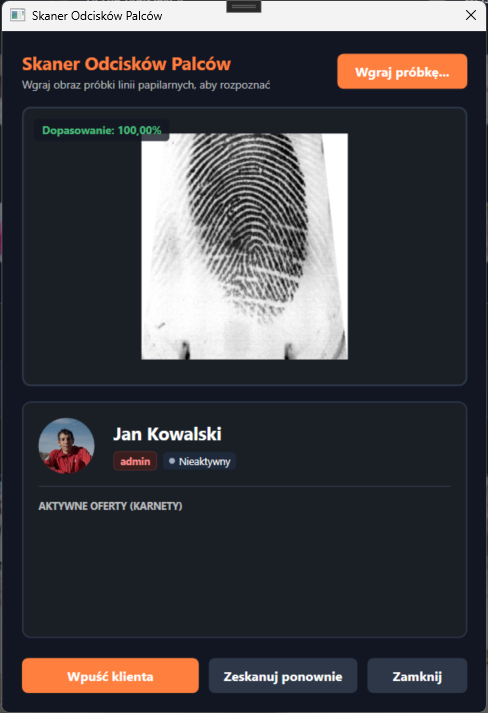
\includegraphics[width=0.40\textwidth]{figures/widoki/FingerprintScannerWindow_succes.png}
    \caption{Pomyślne rozpoznanie i aktywacja wejścia na obiekt}
    \label{fig:finger_scan_success}
\end{figure}

Gdy palec połączony jest z niezidentyfikowanym bądź błędnym wpisem, system wyświetla informacje o braku dostępu.
\begin{figure}[H]
    \centering
    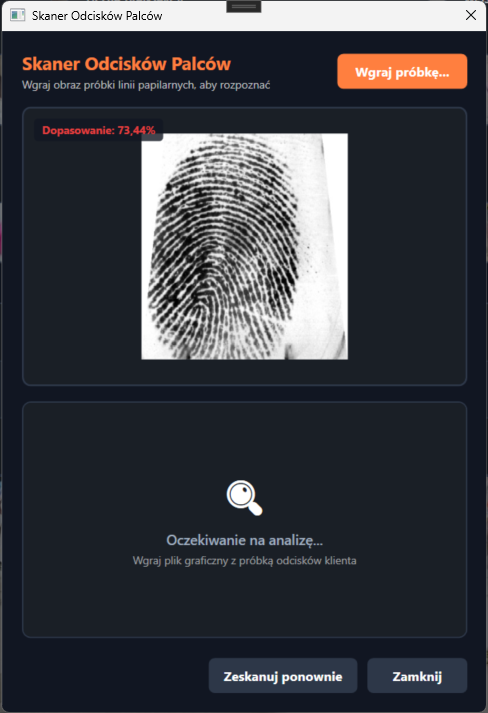
\includegraphics[width=0.40\textwidth]{figures/widoki/FingerprintScannerWindow_error.png}
    \caption{Odrzucenie weryfikacji po przyłożeniu nieznanego odcisku}
    \label{fig:finger_scan_error}
\end{figure}

\newpage
\subsection{Scenariusz 2: Wejście weryfikowane kodem QR}
Jako alternatywę zaprojektowano weryfikację przy użyciu kodów QR, korzystając z wbudowanej w urządzenie kamery.

\begin{figure}[H]
    \centering
    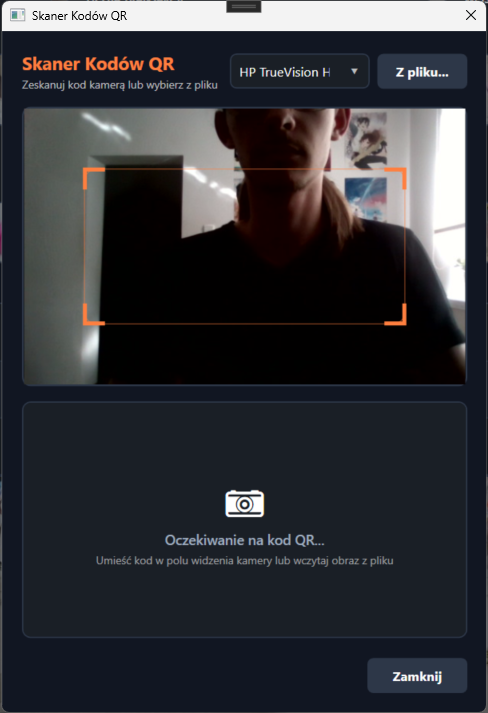
\includegraphics[width=0.40\textwidth]{figures/widoki/QrScannerWindow.png}
    \caption{Czytnik kodów QR w trakcie pracy kamery}
    \label{fig:qr_scan_wait}
\end{figure}

Poprawne zdekodowanie kodu QR z kamery i odnalezienie klienta skutkuje wpuszczeniem klienta na ściankę wspinaczkową oraz zmieniem jego statusu na 'Aktywny'.
\begin{figure}[H]
    \centering
    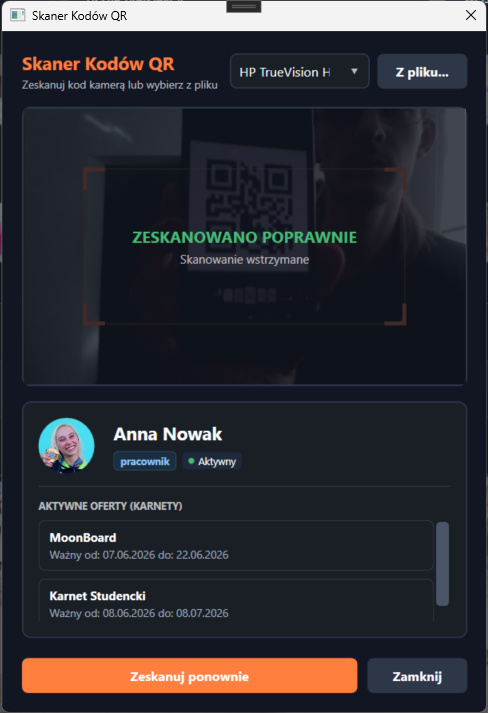
\includegraphics[width=0.40\textwidth]{figures/widoki/QrScannerWindow_succes.png}
    \caption{Pomyślne odczytanie kodu QR i weryfikacja w systemie}
    \label{fig:qr_scan_success}
\end{figure}

Błędny bądź uszkodzony kod wyświetla informację o braku dostępu.
\begin{figure}[H]
    \centering
    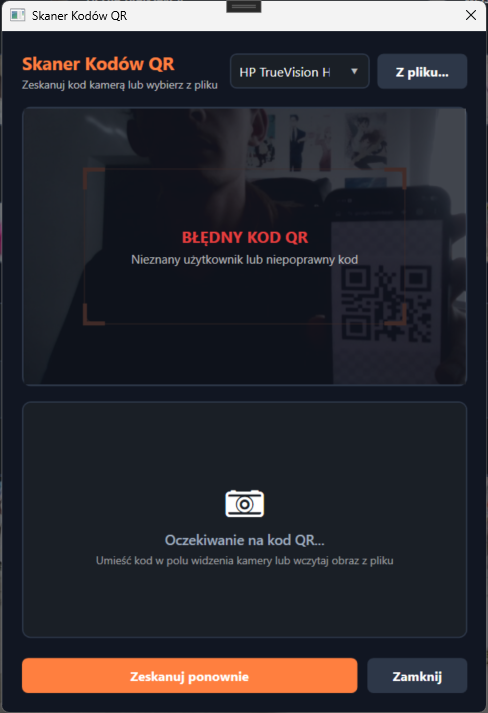
\includegraphics[width=0.40\textwidth]{figures/widoki/QrScannerWindow_error.png}
    \caption{Błąd weryfikacji ze skanera QR}
    \label{fig:qr_scan_error}
\end{figure}
